\chapter{\IfLanguageName{dutch}{Stand van zaken}{State of the art}}%
\label{ch:stand-van-zaken}

Dit hoofdstuk bouwt verder op de inleiding door het onderzoeksdomein theoretisch te kaderen. Waar in het vorige hoofdstuk de concrete casus van Hanuman en de onderzoeksvraag werden geïntroduceerd, wordt hier de bredere academische context besproken. Eerst wordt ERP theoretisch gedefinieerd en gepositioneerd binnen digitale transformatie. Vervolgens worden kritische succesfactoren en risico’s bij ERP-implementaties besproken, met specifieke aandacht voor KMO’s. Daarna wordt het belang van business process reengineering, change management en datakwaliteit toegelicht. Tot slot wordt de Belgische context rond e-invoicing en Peppol besproken.

\section{Enterprise Resource Planning (ERP)}

Enterprise Resource Planning-systemen (ERP) worden in de literatuur omschreven als geïntegreerde informatiesystemen die bedrijfsprocessen over functionele domeinen heen standaardiseren en verbinden \textcite{Davenport1998}. In tegenstelling tot gefragmenteerde softwareoplossingen combineren ERP-systemen modules zoals verkoop, voorraadbeheer, boekhouding en productie in één centrale databank. Hierdoor ontstaat één consistente bron van waarheid voor organisatorische data.

Volgens \textcite{Umble2003} ligt de kernwaarde van ERP in procesintegratie en informatiestroomoptimalisatie. Door standaardisatie van processen en gegevensstructuren kunnen organisaties efficiënter werken en fouten reduceren. ERP-implementaties impliceren echter vaak fundamentele organisatorische veranderingen, omdat bestaande werkmethodes moeten worden aangepast aan het systeemontwerp \autocite{Davenport1998}.

Binnen de context van digitale transformatie wordt ERP beschouwd als een structurele bouwsteen voor schaalbaarheid en procesautomatisering \autocite{Matt2015}. Digitale transformatie overstijgt louter technologie en omvat strategische heroriëntatie, procesherontwerp en cultuurverandering \autocite{Vial2019}. ERP-systemen fungeren hierbij als enabler van geïntegreerde data-analyse en procescontrole.

\section{ERP-implementatie en kritische succesfactoren}

Hoewel ERP aanzienlijke voordelen kan bieden, tonen studies aan dat implementaties gepaard gaan met aanzienlijke risico’s. \textcite{Aloini2007} identificeren risicofactoren zoals onvoldoende projectplanning, gebrekkige gebruikersbetrokkenheid en onderschatting van organisatorische impact.

Een van de meest geciteerde modellen rond kritische succesfactoren is dat van \textcite{Nah2001}. Zij benadrukken onder meer:
\begin{itemize}
    \item topmanagementondersteuning,
    \item duidelijke projectdoelstellingen,
    \item effectieve communicatie,
    \item change management,
    \item en adequaat projectmanagement.
\end{itemize}

Ook \textcite{Somers2001} stellen dat succesfactoren variëren per implementatiefase. In vroege fases ligt de nadruk op planning en scopebepaling, terwijl in latere fases training en gebruikersacceptatie cruciaal worden.

Voor KMO’s zijn deze factoren nog belangrijker, omdat zij beschikken over beperkte middelen en minder gespecialiseerde IT-afdelingen. \textcite{Haddara2012} wijzen erop dat ERP-implementaties in KMO’s vaak mislukken door overschatting van interne capaciteiten en onderschatting van verandermanagement.

\section{ERP in kleine en middelgrote ondernemingen (KMO’s)}

KMO’s verschillen fundamenteel van grote ondernemingen in schaal, complexiteit en middelen. Volgens \textcite{Snider2009} hebben KMO’s doorgaans minder formele processen, sterk gecentraliseerde besluitvorming, beperkte IT-expertise en beperkte budgettaire ruimte.

Dit maakt hen enerzijds flexibeler, maar anderzijds kwetsbaarder bij grootschalige IT-projecten. \textcite{Haddara2012} benadrukken dat standaard ERP-methodologieën vaak onvoldoende aangepast zijn aan KMO-contexten.

Gefaseerde implementatie wordt in meerdere studies naar voren geschoven als risicobeperkende strategie \autocite{Aloini2007}. Door modules stapsgewijs te activeren kan organisatorische weerstand beperkt worden en kan men leren uit tussentijdse evaluaties.

\section{Migratie van losse tools naar een geïntegreerd ERP-systeem}

Veel KMO’s starten hun digitaliseringstraject vanuit een versnipperde IT-omgeving waarin Excel, e-mail, Word-documenten en afzonderlijke boekhoudpakketten naast elkaar bestaan. Dergelijke oplossingen zijn laagdrempelig en flexibel in een beginfase, maar worden problematisch wanneer het aantal klanten, producten, facturen en interne processen toeneemt. Informatie wordt dan verspreid opgeslagen, waardoor dubbele invoer, foutgevoelige berekeningen en beperkte traceerbaarheid ontstaan.

Een ERP-migratie heeft in deze context niet enkel als doel om bestaande documenten te digitaliseren, maar om de onderliggende processen te integreren. Waar Excel vooral geschikt is voor afzonderlijke lijsten of berekeningen, ondersteunt een ERP-systeem procesketens waarbij klantgegevens, offertes, leveringen, voorraadmutaties, facturen en betalingen aan elkaar gekoppeld worden. Dit sluit aan bij de visie van \textcite{Davenport1998}, die ERP-systemen beschrijft als systemen die informatie en processen over functionele domeinen heen verbinden.

De overgang van losse tools naar ERP creëert echter ook risico’s. Bestaande data moet opgeschoond, gestandaardiseerd en gemigreerd worden. Foutieve klantgegevens, ontbrekende btw-nummers, inconsistente productcodes of onvolledige voorraadstanden kunnen leiden tot foutieve facturen, voorraadverschillen of validatiefouten bij elektronische facturatie. Dit maakt data governance en master data management cruciale randvoorwaarden voor een succesvolle migratie \autocite{Umble2003}.

Voor Belgische KMO’s wordt deze uitdaging versterkt door de verplichting tot gestructureerde elektronische B2B-facturatie vanaf 1 januari 2026. Een PDF-factuur of manuele facturatieflow volstaat dan niet langer voor binnenlandse transacties tussen btw-plichtige ondernemingen \autocite{BelgiumEInvoice_2026}. Ondernemingen die vandaag nog sterk afhankelijk zijn van Excel en e-mail moeten daarom niet alleen hun interne efficiëntie verbeteren, maar ook voldoen aan nieuwe externe compliancevereisten.

In de context van Hanuman BV betekent dit dat een ERP-migratie zowel een operationele als een juridische relevantie heeft. De migratie naar Odoo moet enerzijds leiden tot minder manuele handelingen, betere traceerbaarheid en real-time inzicht in voorraad en facturatie. Anderzijds moet het systeem correct worden geconfigureerd om elektronische facturen via Peppol te kunnen genereren en verwerken.

\section{Open-source ERP versus proprietaire systemen}

Binnen de ERP-markt bestaat een onderscheid tussen proprietaire en open-source systemen. Proprietaire systemen werken met licentiemodellen en vaste standaardprocessen. Open-source ERP-systemen bieden meer flexibiliteit in configuratie en aanpassing.

Hoewel open-source oplossingen aantrekkelijk zijn voor KMO’s vanwege lagere instapkosten en flexibiliteit \autocite{Haddara2012}, verschuift het risico naar interne expertise en implementatiecapaciteit. De literatuur rond ERP-risico’s benadrukt dat onvoldoende begeleiding en onduidelijke scope belangrijke faalfactoren vormen \autocite{Aloini2007}.

De keuze voor een open-source systeem zoals Odoo moet daarom niet enkel technologisch maar ook organisatorisch verantwoord worden.

\section{Business Process Reengineering (BPR)}

ERP-implementatie zonder procesherontwerp leidt zelden tot optimale resultaten. \textcite{Hammer1993} stellen dat technologie slechts effectief is wanneer onderliggende processen worden hertekend. Dit concept staat bekend als Business Process Reengineering (BPR).

Volgens \textcite{Davenport1990} vereist procesherontwerp analyse van de huidige situatie (AS-IS), identificatie van inefficiënties en ontwerp van toekomstige processen (TO-BE). ERP moet dus niet enkel bestaande Excel-workflows digitaliseren, maar processen herstructureren op basis van geïntegreerde systeemlogica.

\section{Change Management}

Naast technische implementatie speelt de menselijke factor een cruciale rol. \textcite{Kotter1996} benadrukt dat organisatieverandering vaak faalt door gebrek aan urgentiebesef en onvoldoende communicatie.

ERP-projecten beïnvloeden dagelijkse werkmethodes, verantwoordelijkheden en informatiestromen. Volgens \textcite{Nah2001} is training en gebruikersbetrokkenheid essentieel voor succesvolle adoptie. In kleine ondernemingen waar medewerkers meerdere rollen combineren, is deze factor nog relevanter.

\section{Data governance en stamdatakwaliteit}

Een geïntegreerd ERP-systeem functioneert slechts optimaal wanneer de onderliggende data correct en consistent is. \textcite{Umble2003} benadrukken dat gebrekkige master data kan leiden tot fouten in rapportering, facturatie en voorraadbeheer.

Binnen de context van e-invoicing wordt datakwaliteit nog kritischer. Gestructureerde elektronische facturen vereisen correcte btw-identificatie en conformiteit met standaardformaten \autocite{EuropeanCommission_2025}. Onvolledige of foutieve stamdata kan leiden tot validatiefouten binnen het Peppol-netwerk.

Migratie naar ERP biedt een opportuniteit om data te centraliseren en te standaardiseren, maar verhoogt tegelijk de complexiteit van het implementatieproces.

\section{Procesperformantie en KPI-meting}

Succesvolle ERP-implementatie vereist meetbare doelstellingen. \textcite{Nah2001} benadrukken dat duidelijke evaluatiemetrics essentieel zijn.

Procesperformantie kan gemeten worden via indicatoren zoals:
\begin{itemize}
    \item doorlooptijd,
    \item aantal manuele handelingen,
    \item foutpercentage,
    \item openstaande posten.
\end{itemize}

Volgens \textcite{Davenport1990} moet informatietechnologie leiden tot aantoonbare procesverbetering. Zonder vergelijking tussen AS-IS en TO-BE situatie blijft het effect van ERP moeilijk objectief aantoonbaar.

\section{E-invoicing en Peppol in België}

Naast interne procesoptimalisatie speelt externe compliance een belangrijke rol. De Belgische overheid verplicht vanaf 1 januari 2026 gestructureerde B2B e-facturatie via Peppol \autocite{Deloitte_2024,VLAIO2025}. Deze verplichting kadert binnen een Europese interoperabiliteitsstrategie \autocite{EuropeanCommission_2025}.

Peppol maakt gebruik van gestandaardiseerde elektronische documentuitwisseling. Dit vereist correcte stamdata, validatie van factuurstructuren en technische koppeling met access points.

Peppol werkt volgens een zogenaamd four-corner model. Daarbij communiceren verzender en ontvanger niet rechtstreeks met elkaar, maar via hun respectieve access points. Dit betekent dat een onderneming slechts met één Peppol-serviceprovider moet verbinden om documenten te kunnen uitwisselen met andere deelnemers binnen het netwerk. Voor KMO’s verlaagt dit de technische complexiteit, omdat er geen afzonderlijke koppeling per klant of leverancier nodig is \autocite{OpenPeppolFramework_2026}.

\begin{figure}[H]
    \centering
    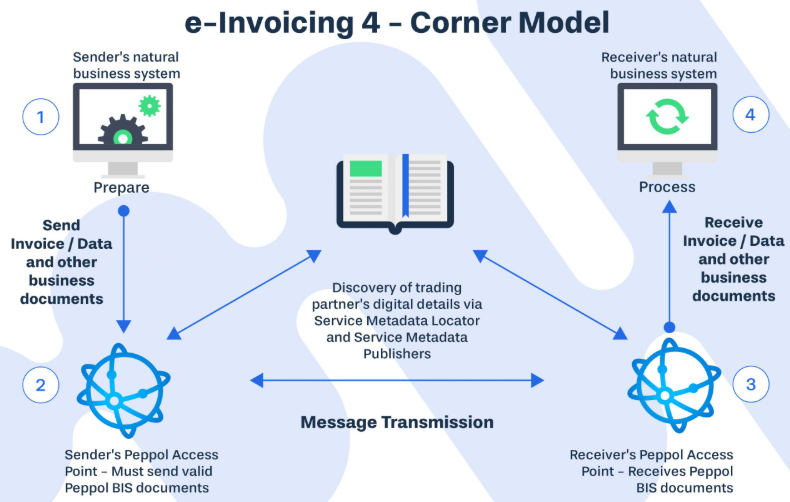
\includegraphics[width=0.85\textwidth]{../graphics/peppol-model.png}
    \caption{Het Peppol four-corner model voor elektronische documentuitwisseling. Bron: OpenPeppol \autocite{OpenPeppolFramework_2026}.}
    \label{fig:peppol-four-corner}
\end{figure}

Voor KMO’s die vandaag nog met manuele facturatie werken, impliceert dit een structurele digitaliseringssprong. ERP-systemen met geïntegreerde e-invoicingfunctionaliteit kunnen deze overgang faciliteren, mits correcte configuratie en procesalignering.

\section{Positionering van Odoo binnen het ERP-landschap}

Binnen het spectrum van open-source ERP-systemen neemt Odoo een bijzondere positie in als modulair en schaalbaar platform dat relevant is voor kleine en middelgrote ondernemingen. Odoo integreert bedrijfsapplicaties zoals CRM, Sales, Inventory, Accounting, Invoicing en Purchase binnen één omgeving \autocite{OdooApps2026}. In tegenstelling tot traditionele, grootschalige ERP-systemen met zware implementatietrajecten, werkt Odoo met een modulair activeringsmodel waarbij functionaliteiten afzonderlijk kunnen worden geïmplementeerd.

\begin{figure}[H]
    \centering
    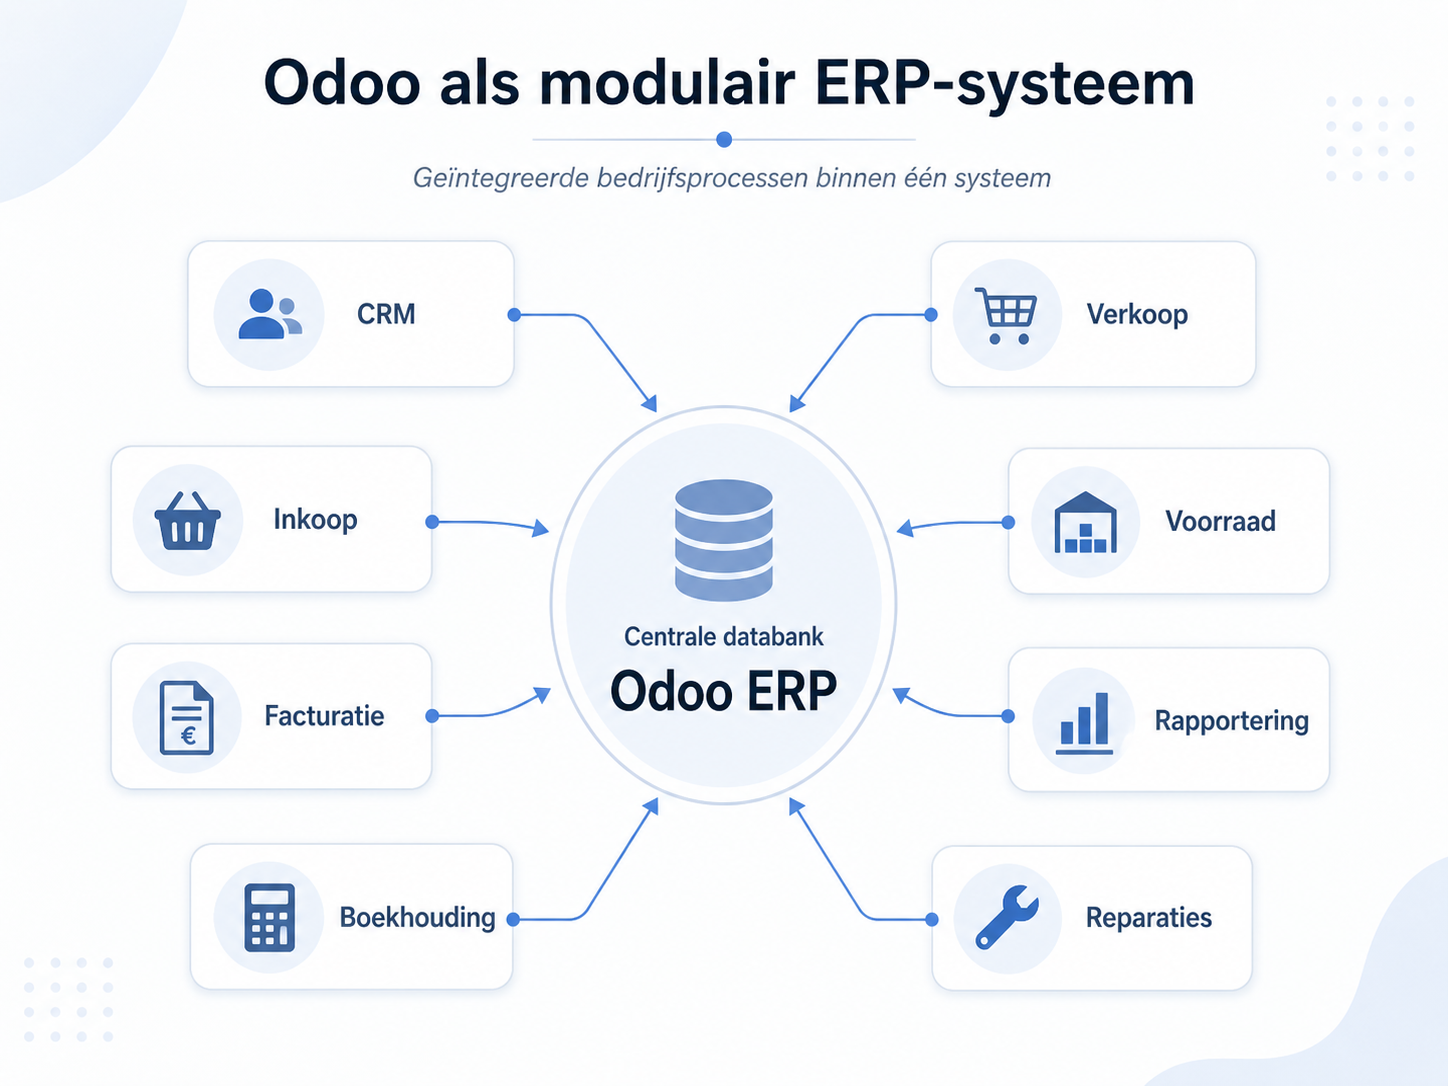
\includegraphics[width=0.85\textwidth]{../graphics/odoo-modules.png}
    \caption{Conceptuele voorstelling van Odoo als modulair ERP-systeem met centrale databank.}
    \label{fig:odoo-module-integratie}
\end{figure}

Deze modulaire structuur is relevant voor KMO’s omdat ERP-implementaties vaak beperkt worden door budget, interne expertise en veranderingscapaciteit. Een onderneming hoeft niet noodzakelijk in één keer een volledig ERP-systeem te implementeren, maar kan starten met kritieke processen zoals verkoop en facturatie. Nadien kunnen voorraadbeheer, aankoop, reparatiebeheer en rapportering stapsgewijs worden toegevoegd.

Dit sluit aan bij de literatuur die gefaseerde implementatie aanbeveelt als risicobeperkende strategie in KMO-context \autocite{Aloini2007,Haddara2012}. Door modules stapsgewijs te activeren kan organisatorische weerstand worden beperkt en kan iteratief worden bijgestuurd op basis van praktijkervaring.

Binnen de Belgische KMO-context bestaan naast Odoo ook alternatieven zoals Exact Online, Teamleader en Microsoft Dynamics 365 Business Central. Exact Online positioneert zich sterk rond boekhouding, financiële administratie en e-invoicing, en biedt Peppol-functionaliteit aan binnen zijn oplossingen \autocite{ExactOnline2026,ExactPeppol2026}. Teamleader focust vooral op CRM, offertes, facturatie en projectopvolging voor kleinere ondernemingen \autocite{Teamleader2026}. Microsoft Dynamics 365 Business Central biedt een breder ERP-platform voor kleine en middelgrote ondernemingen, met functionaliteiten voor financiën, verkoop en operations \autocite{MicrosoftBusinessCentral2026}.

Voor de case van Hanuman BV is Odoo bijzonder relevant omdat het meerdere noodzakelijke bedrijfsprocessen combineert binnen één modulair platform: verkoop, facturatie, voorraadbeheer, aankoop, klantenbeheer en repair/service-opvolging. Daarnaast biedt Odoo documentatie en functionaliteit rond elektronische facturatie en Peppol, wat aansluit bij de Belgische verplichting rond gestructureerde B2B-e-facturatie \autocite{OdooPeppolBelgium2026,OdooEInvoicingDocs2026}. Daardoor sluit Odoo goed aan bij de combinatie van procesintegratie, gefaseerde implementatie en Peppol-readiness die in deze bachelorproef centraal staat.

Tegelijk betekent de flexibiliteit van Odoo niet dat implementatie zonder voorbereiding kan gebeuren. Landenspecifieke configuratie, fiscale localisatie en elektronische facturatie zijn afhankelijk van correcte bedrijfsgegevens, btw-instellingen en boekhoudkundige configuratie. Voor Belgische ondernemingen is dit extra belangrijk, omdat e-invoicing en Peppol-integratie rechtstreeks afhankelijk zijn van correcte stamdata zoals btw-nummers, adressen, bankrekeningen en Peppol-identificatoren.

De keuze voor Odoo in deze bachelorproef is dan ook geen louter technische voorkeur, maar een onderzoeksmatig gefundeerde selectie van een open-source ERP-platform dat aansluit bij de schaal, middelen en flexibiliteitsvereisten van een servicegerichte Belgische KMO zoals Hanuman BV.

\section{Synthese en positionering van het onderzoek}

De literatuur toont aan dat ERP-systemen krachtige instrumenten zijn voor procesintegratie en digitale transformatie \autocite{Davenport1998,Matt2015}. Tegelijkertijd wijzen talrijke studies op significante implementatierisico’s, vooral in KMO-contexten \autocite{Nah2001,Haddara2012,Aloini2007}.

Succesvolle implementatie vereist:
\begin{itemize}
    \item gefaseerde aanpak,
    \item procesherontwerp,
    \item sterk change management,
    \item aandacht voor datakwaliteit,
    \item en expliciete KPI-meting.
\end{itemize}

De verplichte Peppol-e-invoicing verhoogt de urgentie van digitale integratie in Belgische ondernemingen \autocite{Deloitte_2024}. Dit creëert een unieke combinatie van interne efficiëntieverbetering en externe compliancevereisten.

Deze bachelorproef positioneert zich binnen dit theoretisch kader als een praktijkgerichte casestudy die onderzoekt hoe een gefaseerde ERP-migratie in een servicegerichte KMO kan leiden tot meetbare procesverbetering en e-invoicing-readiness. Daarbij ligt de nadruk niet op een volledige productie-uitrol, maar op het ontwerpen en evalueren van een reproduceerbaar migratiekader voor Odoo binnen een gecontroleerde casuscontext.